\ifnum \Version=1    
    \question[1] You do not need to show your work for this question. Consider the nonlinear system below.
    \begin{align*}
        \dxdt &= (x-1)(y-2) , \qquad \dydt = (x-3)(y-1)
    \end{align*}
    How many critical points does the system have? \framebox{\strut\hspace{1cm}}
    \ifnum \Solutions=1 {\color{DarkBlue} \\[12pt] 
    For a point to critical point, we need $x' = y' = 0$. If $x'$ is zero, then either $x=1$ or $y=2$. Likewise if $y'=0$ then $x=3$ or $y=1$. The lines are shown below. The green lines are the x nullclines, and the red lines are the y nullclines. There are exactly two critical points. 
        \begin{center}
        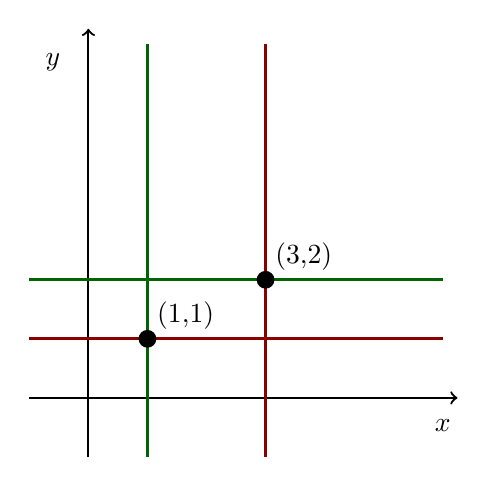
\begin{tikzpicture}[scale=0.75]
        \draw[thick, ->] (-1, 0) -- (6.25, 0);
        \draw[thick, ->] (0, -1) -- (0, 6.25);
        \node[overlay, below] at (6, -0.2) {$x$};
        \node[overlay, below] at (-0.6, 6) {$y$};   
        \draw[very thick,DarkGreen, -] (1, 6) -- (1, -1);        
        \draw[very thick,DarkGreen, -] (-1, 2) -- (6, 2);   
        \draw[very thick,DarkRed, -] (3, 6) -- (3, -1);        
        \draw[very thick,DarkRed, -] (6, 1) -- (-1, 1);      
        \filldraw[black] (1,1) circle (4pt) node[anchor=south west]{(1,1)};
        \filldraw[black] (3,2) circle (4pt) node[anchor=south west]{(3,2)};
        \end{tikzpicture}
        \end{center}         
    } 
    \else 
    \vspace{0.5cm}
    \fi    
\fi 


\ifnum \Version=6
\question[2] Consider the following IVP: $y' = y + t+1$, $y(0) = 6$. Use the Euler method to estimate $y(1)$ with step size $h=0.5$.

\ifnum \Solutions=1 {\color{DarkBlue} 
\textbf{Solutions:} We need two iterations to approximate the solution to the initial value problem (IVP) using Euler's method with a step size of \( h = 0.5 \).

\begin{itemize}
    \item Calculate $y_1$. 
        \begin{align}
            t_0 &= 0 \\
            y_0 &= 6 \\
            f(t_0, y_0) &= y_0 + t_0 + 1 = 7 \\
            y_1 &= y_0 + h f(t_0, y_0) = 6 +3.5 = 9.5
        \end{align}
            
    \item Calculate \( y_2 \).
        \begin{align}
            t_1 &= t_0 + h = 0 + 0.5 = 0.5 \\
            y_1 &= 9.5 \\
            f(t_1, y_1) &= y_1 + t_1 + 1 = 9.5 + 0.5 + 1 = 11 \\
          y_2 &= y_1 + h f(t_1, y_1) = 9.5 + 0.5 \cdot 11 = 15
        \end{align} 
\end{itemize}

The estimated value of \( y(1) \) is \( 15 \) using Euler's method with a step size of \( h = 0.5 \).
} 
\else 
\newpage
\fi
\fi 


\ifnum \Version=7
\question[2] Consider the following IVP: $y' = y + 2t+4$, $y(0) = 2$. Use the Euler method to estimate $y(1)$ with step size $h=0.5$.

\ifnum \Solutions=1 {\color{DarkBlue} 
\textbf{Solutions:} We need two iterations to approximate the solution to the initial value problem (IVP) using Euler's method with a step size of \( h = 0.5 \).

\begin{itemize}
    \item Calculate $y_1$. 
        \begin{align}
            t_0 &= 0 \\
            y_0 &= 2 \\
            f(t_0, y_0) &= y_0 + 2t_0 + 4 = 6 \\
            y_1 &= y_0 + h f(t_0, y_0) = 2 + 0.5 \cdot 6 = 5
        \end{align}
            
    \item Calculate \( y_2 \).
        \begin{align}
            t_1 &= t_0 + h = 0 + 0.5 = 0.5 \\
            y_1 &= 5 \\
            f(t_1, y_1) &= y_1 + 2 t_1 + 4 = 5 + 2\cdot 0.5 + 4 = 10 \\
          y_2 &= y_1 + h f(t_1, y_1) = 5 + 0.5 \cdot 10 = 10
        \end{align} 
\end{itemize}

The estimated value of \( y(1) \) is \( 10 \) using Euler's method with a step size of \( h = 0.5 \).
} 
\else 
\newpage
\fi
\fi 